


\tikzset{every picture/.style={line width=0.75pt}} %set default line width to 0.75pt        

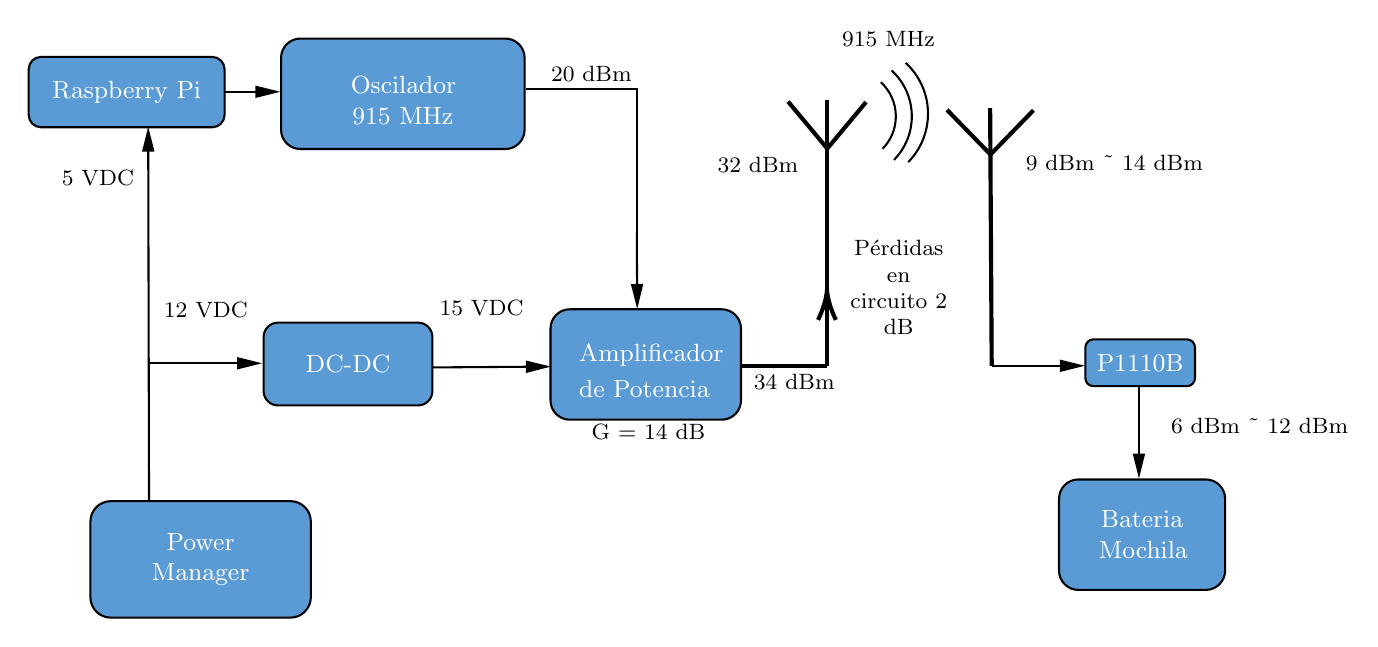
\begin{tikzpicture}[x=0.75pt,y=0.75pt,yscale=-1,xscale=1]
%uncomment if require: \path (0,302); %set diagram left start at 0, and has height of 302

%Flowchart: Alternative Process [id:dp5901024681209728] 
\draw  [color={rgb, 255:red, 0; green, 0; blue, 0 }  ,draw opacity=1 ][fill={rgb, 255:red, 91; green, 155; blue, 213 }  ,fill opacity=1 ] (3.83,23.53) .. controls (3.83,20.26) and (6.49,17.6) .. (9.76,17.6) -- (92.25,17.6) .. controls (95.52,17.6) and (98.18,20.26) .. (98.18,23.53) -- (98.18,45.56) .. controls (98.18,48.84) and (95.52,51.49) .. (92.25,51.49) -- (9.76,51.49) .. controls (6.49,51.49) and (3.83,48.84) .. (3.83,45.56) -- cycle ;
%Flowchart: Alternative Process [id:dp9678129498459402] 
\draw  [color={rgb, 255:red, 0; green, 0; blue, 0 }  ,draw opacity=1 ][fill={rgb, 255:red, 91; green, 155; blue, 213 }  ,fill opacity=1 ] (125.4,18.07) .. controls (125.4,12.93) and (129.57,8.76) .. (134.71,8.76) -- (233.44,8.76) .. controls (238.58,8.76) and (242.75,12.93) .. (242.75,18.07) -- (242.75,52.66) .. controls (242.75,57.81) and (238.58,61.98) .. (233.44,61.98) -- (134.71,61.98) .. controls (129.57,61.98) and (125.4,57.81) .. (125.4,52.66) -- cycle ;
%Flowchart: Alternative Process [id:dp03056880673326523] 
\draw  [color={rgb, 255:red, 0; green, 0; blue, 0 }  ,draw opacity=1 ][fill={rgb, 255:red, 91; green, 155; blue, 213 }  ,fill opacity=1 ] (33.56,241.45) .. controls (33.56,236.03) and (37.96,231.63) .. (43.38,231.63) -- (129.93,231.63) .. controls (135.35,231.63) and (139.75,236.03) .. (139.75,241.45) -- (139.75,277.93) .. controls (139.75,283.35) and (135.35,287.75) .. (129.93,287.75) -- (43.38,287.75) .. controls (37.96,287.75) and (33.56,283.35) .. (33.56,277.93) -- cycle ;
%Flowchart: Alternative Process [id:dp843232670273814] 
\draw  [color={rgb, 255:red, 0; green, 0; blue, 0 }  ,draw opacity=1 ][fill={rgb, 255:red, 91; green, 155; blue, 213 }  ,fill opacity=1 ] (117,152.59) .. controls (117,148.73) and (120.13,145.6) .. (123.99,145.6) -- (191.36,145.6) .. controls (195.21,145.6) and (198.34,148.73) .. (198.34,152.59) -- (198.34,178.53) .. controls (198.34,182.39) and (195.21,185.52) .. (191.36,185.52) -- (123.99,185.52) .. controls (120.13,185.52) and (117,182.39) .. (117,178.53) -- cycle ;
%Flowchart: Alternative Process [id:dp2196391995059177] 
\draw  [color={rgb, 255:red, 0; green, 0; blue, 0 }  ,draw opacity=1 ][fill={rgb, 255:red, 91; green, 155; blue, 213 }  ,fill opacity=1 ] (255.23,148.49) .. controls (255.23,143.35) and (259.4,139.18) .. (264.54,139.18) -- (337.69,139.18) .. controls (342.83,139.18) and (347,143.35) .. (347,148.49) -- (347,183.08) .. controls (347,188.22) and (342.83,192.39) .. (337.69,192.39) -- (264.54,192.39) .. controls (259.4,192.39) and (255.23,188.22) .. (255.23,183.08) -- cycle ;
%Straight Lines [id:da7648549186794515] 
\draw [line width=1.5]    (346.74,166.51) -- (388.43,166.51) ;
%Straight Lines [id:da35576594493962777] 
\draw [line width=1.5]    (388.43,166.51) -- (388.43,133.09) ;
\draw [shift={(388.43,130.09)}, rotate = 450] [color={rgb, 255:red, 0; green, 0; blue, 0 }  ][line width=1.5]    (14.21,-4.28) .. controls (9.04,-1.82) and (4.3,-0.39) .. (0,0) .. controls (4.3,0.39) and (9.04,1.82) .. (14.21,4.28)   ;
%Straight Lines [id:da02646954268865498] 
\draw [line width=1.5]    (388.43,38.25) -- (388.43,130.09) ;
%Straight Lines [id:da4914114624712449] 
\draw [line width=1.5]    (369.69,39.12) -- (388.58,61.75) ;
%Straight Lines [id:da9035567772895365] 
\draw [line width=1.5]    (388.58,61.75) -- (407.25,39.38) ;

%Shape: Arc [id:dp5933295871897399] 
\draw  [draw opacity=0] (419.61,24.16) .. controls (425.61,29.68) and (429.35,37.62) .. (429.3,46.42) .. controls (429.25,54.52) and (425.99,61.86) .. (420.73,67.23) -- (399.3,46.23) -- cycle ; \draw   (419.61,24.16) .. controls (425.61,29.68) and (429.35,37.62) .. (429.3,46.42) .. controls (429.25,54.52) and (425.99,61.86) .. (420.73,67.23) ;
%Shape: Arc [id:dp846123263641188] 
\draw  [draw opacity=0] (414.41,29.82) .. controls (418.87,33.93) and (421.65,39.83) .. (421.61,46.37) .. controls (421.57,52.4) and (419.15,57.85) .. (415.24,61.84) -- (399.3,46.23) -- cycle ; \draw   (414.41,29.82) .. controls (418.87,33.93) and (421.65,39.83) .. (421.61,46.37) .. controls (421.57,52.4) and (419.15,57.85) .. (415.24,61.84) ;
%Shape: Arc [id:dp3021222167053754] 
\draw  [draw opacity=0] (426.35,20.47) .. controls (433.01,26.6) and (437.16,35.4) .. (437.1,45.17) .. controls (437.04,54.16) and (433.42,62.3) .. (427.59,68.26) -- (403.81,44.96) -- cycle ; \draw   (426.35,20.47) .. controls (433.01,26.6) and (437.16,35.4) .. (437.1,45.17) .. controls (437.04,54.16) and (433.42,62.3) .. (427.59,68.26) ;
%Straight Lines [id:da9393977842068026] 
\draw [line width=1.5]    (467.04,42.25) -- (467.8,166.4) ;
%Straight Lines [id:da6609719078207286] 
\draw [line width=1.5]    (446.25,43.08) -- (467.2,64.62) ;
%Straight Lines [id:da1212283700039476] 
\draw [line width=1.5]    (467.2,64.62) -- (487.9,43.32) ;
%Flowchart: Alternative Process [id:dp07927580495302378] 
\draw  [color={rgb, 255:red, 0; green, 0; blue, 0 }  ,draw opacity=1 ][fill={rgb, 255:red, 91; green, 155; blue, 213 }  ,fill opacity=1 ] (512.93,157.61) .. controls (512.93,155.43) and (514.69,153.66) .. (516.88,153.66) -- (561.8,153.66) .. controls (563.98,153.66) and (565.75,155.43) .. (565.75,157.61) -- (565.75,172.3) .. controls (565.75,174.48) and (563.98,176.25) .. (561.8,176.25) -- (516.88,176.25) .. controls (514.69,176.25) and (512.93,174.48) .. (512.93,172.3) -- cycle ;
%Flowchart: Alternative Process [id:dp4035191156494293] 
\draw  [color={rgb, 255:red, 0; green, 0; blue, 0 }  ,draw opacity=1 ][fill={rgb, 255:red, 91; green, 155; blue, 213 }  ,fill opacity=1 ] (500.23,230.49) .. controls (500.23,225.35) and (504.4,221.18) .. (509.54,221.18) -- (570.94,221.18) .. controls (576.08,221.18) and (580.25,225.35) .. (580.25,230.49) -- (580.25,265.08) .. controls (580.25,270.22) and (576.08,274.39) .. (570.94,274.39) -- (509.54,274.39) .. controls (504.4,274.39) and (500.23,270.22) .. (500.23,265.08) -- cycle ;
%Straight Lines [id:da744994327328814] 
\draw    (538.75,176.75) -- (538.75,218.75) ;
\draw [shift={(538.75,220.75)}, rotate = 270] [fill={rgb, 255:red, 0; green, 0; blue, 0 }  ][line width=0.08]  [draw opacity=0] (12,-3) -- (0,0) -- (12,3) -- cycle    ;
%Straight Lines [id:da8045553258070812] 
\draw    (198.6,167.2) -- (253.4,166.81) ;
\draw [shift={(255.4,166.8)}, rotate = 539.6] [fill={rgb, 255:red, 0; green, 0; blue, 0 }  ][line width=0.08]  [draw opacity=0] (12,-3) -- (0,0) -- (12,3) -- cycle    ;
%Straight Lines [id:da7341411358280834] 
\draw    (61.8,231.6) -- (61.4,53.2) ;
\draw [shift={(61.4,51.2)}, rotate = 449.87] [fill={rgb, 255:red, 0; green, 0; blue, 0 }  ][line width=0.08]  [draw opacity=0] (12,-3) -- (0,0) -- (12,3) -- cycle    ;
%Straight Lines [id:da31234262555733583] 
\draw    (61.4,165.2) -- (114.2,165.2) ;
\draw [shift={(116.2,165.2)}, rotate = 180] [fill={rgb, 255:red, 0; green, 0; blue, 0 }  ][line width=0.08]  [draw opacity=0] (12,-3) -- (0,0) -- (12,3) -- cycle    ;
%Straight Lines [id:da4614416028173276] 
\draw    (98.6,34.4) -- (123,34.4) ;
\draw [shift={(125,34.4)}, rotate = 180] [fill={rgb, 255:red, 0; green, 0; blue, 0 }  ][line width=0.08]  [draw opacity=0] (12,-3) -- (0,0) -- (12,3) -- cycle    ;
%Shape: Right Angle [id:dp5998155804613801] 
\draw   (243.4,33) -- (296.8,33) -- (296.8,103) ;
%Straight Lines [id:da3318034540290906] 
\draw    (296.8,102) -- (296.99,137) ;
\draw [shift={(297,139)}, rotate = 269.69] [fill={rgb, 255:red, 0; green, 0; blue, 0 }  ][line width=0.08]  [draw opacity=0] (12,-3) -- (0,0) -- (12,3) -- cycle    ;
%Straight Lines [id:da7436914839494935] 
\draw    (467.8,166.4) -- (510.6,166.4) ;
\draw [shift={(512.6,166.4)}, rotate = 180] [fill={rgb, 255:red, 0; green, 0; blue, 0 }  ][line width=0.08]  [draw opacity=0] (12,-3) -- (0,0) -- (12,3) -- cycle    ;

% Text Node
\draw (184.07,35.37) node  [font=\small,color={rgb, 255:red, 255; green, 255; blue, 255 }  ,opacity=1 ] [align=left] {\begin{minipage}[lt]{37.62pt}\setlength\topsep{0pt}
\begin{center}
{\small Oscilador}\\{\small 915 MHz}
\end{center}

\end{minipage}};
% Text Node
\draw (86.65,259.69) node  [font=\small,color={rgb, 255:red, 255; green, 255; blue, 255 }  ,opacity=1 ] [align=left] {\begin{minipage}[lt]{61.05pt}\setlength\topsep{0pt}
\begin{center}
{\small Power Manager}
\end{center}

\end{minipage}};
% Text Node
\draw (157.67,165.56) node  [font=\small,color={rgb, 255:red, 255; green, 255; blue, 255 }  ,opacity=1 ] [align=left] {{\small DC-DC}};
% Text Node
\draw (301.11,165.78) node  [font=\small,color={rgb, 255:red, 255; green, 255; blue, 255 }  ,opacity=1 ] [align=left] {\begin{minipage}[lt]{48.18pt}\setlength\topsep{0pt}
\begin{center}
{\small Amplificador}
\end{center}
{\small de Potencia}
\end{minipage}};
% Text Node
\draw (539.34,164.96) node  [font=\small,color={rgb, 255:red, 255; green, 255; blue, 255 }  ,opacity=1 ] [align=left] {P1110B};
% Text Node
\draw (51.01,34.55) node  [color={rgb, 255:red, 255; green, 255; blue, 255 }  ,opacity=1 ] [align=left] {{\small Raspberry Pi}};
% Text Node
\draw (540.24,247.78) node  [font=\small,color={rgb, 255:red, 255; green, 255; blue, 255 }  ,opacity=1 ] [align=left] {\begin{minipage}[lt]{31.2pt}\setlength\topsep{0pt}
\begin{center}
{\small Bateria}\\{\small Mochila}
\end{center}

\end{minipage}};
% Text Node
\draw (254,20.47) node [anchor=north west][inner sep=0.75pt]  [font=\footnotesize] [align=left] {20 dBm};
% Text Node
\draw (200.3,133.2) node [anchor=north west][inner sep=0.75pt]  [font=\footnotesize] [align=left] {15 VDC};
% Text Node
\draw (67.5,134.2) node [anchor=north west][inner sep=0.75pt]  [font=\footnotesize] [align=left] {12 VDC};
% Text Node
\draw (18.3,70.7) node [anchor=north west][inner sep=0.75pt]  [font=\footnotesize] [align=left] {5 VDC};
% Text Node
\draw (273.6,193.1) node [anchor=north west][inner sep=0.75pt]   [align=left] {{\footnotesize G = 14 dB}};
% Text Node
\draw (351.74,169.01) node [anchor=north west][inner sep=0.75pt]  [font=\footnotesize] [align=left] {34 dBm};
% Text Node
\draw (395.74,104.51) node [anchor=north west][inner sep=0.75pt]  [font=\footnotesize] [align=left] {\begin{minipage}[lt]{38.64pt}\setlength\topsep{0pt}
\begin{center}
{\footnotesize Pérdidas en}\\{\footnotesize circuito 2 dB}
\end{center}

\end{minipage}};
% Text Node
\draw (334.24,64.51) node [anchor=north west][inner sep=0.75pt]  [font=\footnotesize] [align=left] {32 dBm};
% Text Node
\draw (394.24,4.01) node [anchor=north west][inner sep=0.75pt]  [font=\footnotesize] [align=left] {915 MHz};
% Text Node
\draw (482.74,63.51) node [anchor=north west][inner sep=0.75pt]  [font=\footnotesize] [align=left] {{\footnotesize 9 dBm \textasciitilde \ 14 dBm}};
% Text Node
\draw (552.74,190.01) node [anchor=north west][inner sep=0.75pt]  [font=\footnotesize] [align=left] {{\footnotesize 6 dBm \textasciitilde \ 12 dBm}};


\end{tikzpicture}